\documentclass[11pt, sakura, night, 1in]{hw}
\def\course{CSC240 Winter 2024}
\def\headername{Homework Assignment 9}
\def\name{Joseph Siu}

\usepackage{clsfiles/csc240}
\usepackage[noend, nocap]{clsfiles/alg}
\usepackage{tikz}
\usetikzlibrary{automata,positioning}

\newop{\A}{A}

\begin{document}

1. Consider the following iterative algorithm that finds the length of the longest increasing subsequence in the array $\A[1..n].$

\newalg{
    \as \ag{L[1]}{1}
    \afor{\ag{i}{2}\;\TO\;$n$\;\DO}{
        \as \ag{L[i]}{1}
        \afor{\ag{j}{1}\;\TO\;$i-1$\;\DO}{
            \aif{($A[j] < A[i]$) and ($L[j] \geq L[i]$) then}{
                \ag{L[i]}{L[j] + 1}
            }
        }
    }
    \as \ag{m}{L[n]}
    \afor{\ag{i}{2}\;\TO\;$n-1$\;\DO}{
        \aif{$L[i] > m$ then}{
            \ag{m}{L[i]}
        }
    }
}

(a) Give a precise statement of what it means for this algorithm to be partially correct.

\Precon: $n$ is a positive integer, and $\A[1..n]$ is an array with elements from a totally ordered domain.

\Postcon: The array $\A[1..n]$ is unchanged, and $m$ is assigned with a positive integer which represents the length of the longest increasing subsequence in $\A[1..n]$.

Partially correct: If $n$ is a positive integer $n$, $\A[1..n]$ is an array with elements from a totally ordered domain, and the algorithm is executed and terminated, then $\A[1..n]$ is unchanged, and $m$ is assigned with a positive integer which represents the length of the longest increasing subsequence in $\A[1..n]$. 


(b) Prove that this algorithm is partially correct.

We will use L1, L2 to denote line 1, line 2, and so on.

We also assumed the line numbers of the pseudo-code are fixed (L6, L7, L8 instead of L7, L8, L9).

\tit{Proof of Question 1(b).}

\indenv{
    Assume $n$ is a positive integer, $\A[1..n]$ is an array with elements from a totally ordered domain, and the algorithm is executed and terminated. 
    
    Since there are no assignments to $\A[1..n]$ in the algorithm, $\A[1..n]$ is unchanged.

    For $l\in\N$. Let $Q(l)=``$immediately after the $l^{\T{th}}$ iteration, $L[l+1]$ contains the length of the longest increasing (finite) subsequence in $\A[1..(l+1)]$ that ends with the term $\A[l+1]''$; and let $P(l)$=``If the for-loop from line 2 to line 5 is executed at least $l$ times, then $Q(l)$.'' 

    \tbf{Lemma 1.} $\forall l\in\N. P(l).$

    \tit{Proof of Lemma 1 by strong induction.}

    \indenv{
        Let $l\in\N$ be arbitrary;
        \indenv{
            Assume $\forall k\in\N. (k<l)\iimplies P(k)$.
            \indenv{
                Assume the for-loop from line 2 to line 5 is executed at least $l$ times.

                \begin{proofcases}
                    \case $l=0$. 
                    \indenv{
                        Then trivially the length of the longest increasing subsequence in $\A[1..1]$ is 1, and we assigned $L[1]=1$ on L1. Thus $Q(0)$ holds.
                    }
                    For Case 1 $Q(l)$.

                    \case $l=1$. 
                    \indenv{
                        Then for the first iteration, $i=2$; on L3 $L[2]$ is assigned with 1; on L4 since $j$ is from 1 to $2-1=1$, we only execute L5 once where $j=1$, and there are 2 subcases due to $L[1]=1\ge1=L[2]$:
                    
                        \subcase $A[j]<A[i]$ 
                        \indenv{
                            Then on L5 $L[2]$ is assigned with $L[1]+1=2$, after this we end this iteration, and now $L[2]=2$ is indeed the length of the longest increasing subsequence in $\A[1..2]$. 
                        }

                        Thus $Q(l)$ holds for subcase 2.1.

                        \subcase $A[j]\ge A[i]$. 
                        \indenv{
                            Then no assignment on L5 has been made. After this we end this iteration, and now $L[2]=1$ is indeed the length of the longest increasing subsequence in $\A[1..2]$ since $\A[j]=\A[1]\ge\A[2]=\A[i]$. 
                        }

                        Thus $Q(l)$ holds for subcase 2.2.
                    }
                    
                    For all subcases of Case 2 we have shown $Q(l)$ holds, so for Case 2 $Q(l)$.

                    \case $l\ge2$. 
                    \indenv{
                        We first assign $L[l]=1$ on L3. 
                        
                        Now, let $S=\{p\in[l]\mid A[p]<A[l]\}$, and let $S'=\{L[p]\mid p\in S\}$. 
                        
                        \subcase $S=\emptyset$. 
                        \indenv{
                            Then since for all $p\in[l].\nnot(A[p]<A[l])$, no assignment on L5 has been made, and $L[l+1]=1$ is indeed the length of the longest increasing subsequence in $\A[1..(l+1)]$ with the last term $\A[l+1]$ (all previous terms are at least $\A[l+1]$). 
                        }
                        Thus $Q(l)$ holds for subcase 3.1.

                        \subcase $S\ne\emptyset$. 
                        \indenv{
                            Then by construction this implies $S'\ne\emptyset$.

                            $i=l+1$ on L2.
                            
                            Since $S'$ is a finite non-empty subset of $\Z^+$, we are allowed to construct $q=\max S'$. 
                            
                            Then $q\in S'$, by construction there exists $p'\in S$ such that $q=L[p']$, we instantiate such $p'$. 
                            
                            By inductive hypothesis (specialization and modus ponens), $q$ is the length of the longest increasing subsequence in $\A[1..p']$ that ends with the term $\A[p']$. We instantiate such subsequence as $\{s_o\}_{o=1}^q$. Moreover, because $q=\max S'$, this means $q$ is the length of the longest increasing subsequence in $\A[1..l]$ that ends with a term less than $\A[l]$.

                            Now, we claim the subsequence $\{s_o\}_{o=1}^q\circ\{\A[l+1]\}$ is the longest increasing subsequence in $\A[1..(l+1)]$ that ends with the term $\A[l+1]$. Indeed, firsly for a subsequence to be both increasing and ends with $\A[l+1]$, the term before $\A[l+1]$ must be less than $\A[l+1]$, and by A8 $\{s_o\}_{o=1}^q\circ\{\A[l+1]\}$ is increasing since $\{s_o\}_{o=1}^q$ is increasing and $s_q=\A[p']<\A[l+1]$ by definition of $S$. Secondly, obviously the concatenation shows the subsequence ends with $\A[l+1]$. Lastly, $\{s_o\}_{o=1}^q$ being the longest increasing subsequence in $\A[1..l]$ implies $\{s_o\}_{o=1}^q\circ\{\A[l+1]\}$ is the longest increasing subsequence in $\A[1..(l+1)]$ that ends with the term $\A[l+1]$. 

                            Therefore, as long as we show $L[l+1]=q+1$, we can conclude $Q(l)$ holds.

                            To this end, since $1\le p'\le l=i-1$, for the for-loop from L4 to L5, right after the iteration where $j=p'$, since $A[p']<A[l]$, and $L[p']\ge L[l]$ due to our construction of $q$, on L5 $L[l+1]$ is assigned with $L[p']+1=q+1$. And after this iteration, consider 2 cases:

                            1. If $A[j]<A[l]$, then since $L[x]\le L[p']=L[l+1]$ for all $x\in S'$ by construction of $q$, no assignment on L5 has been made.

                            2. If $A[j]\ge A[l]$, then no assignment on L5 has been made.

                            For both subcases 3.2.1 and 3.2.2, we have shown that immediately after the $l^{\T{th}}$ iteration, $L[l+1]=q+1$ is indeed the length of the longest increasing subsequence in $\A[1..(l+1)]$ that ends with the term $\A[l+1]$. Thus $Q(l)$ holds for subcase 3.2.
                        }
                    }

                    For all subcases of Case 3 we have shown $Q(l)$ holds, so for Case 3 $Q(l)$.
                \end{proofcases}

                For all cases we have shown $Q(l)$ holds, so $Q(l)$.
            }

            By direct proof, $P(l)$.
        }
    }

    By strong induction, $\forall l\in\N. P(l)$. QED.

    Now, since there are no assignments to $i$ and $j$ within their for-loop respectively, and so only finitely many for-loop iterations has performed thus the for loop from L2 to L5 eventually terminates. Now we are on L6.
    
    \begin{proofcases}
        \case $n=1$.
        \indenv{
            Then we assign $m$ with $L[n]=L[1]=1$ and the algorithm terminates. Thus $m$ is assigned with a positive integer which represents the length of the longest increasing subsequence in $\A[1..n]$.
        }
        For Case 1 $m$ is assigned with a positive integer which represents the length of the longest increasing subsequence in $\A[1..n]$.
        \case $n\ge2$.
        \indenv{
            From L6 to L8, we assign $m$ with the largest value in $L[2..n]$, since $L[n]\ge L[1]$, such $m$ is also the largest value in $L[1..n]$. Since by Lemma 1 $L[y]$ is the length of the longest increasing subsequence in $\A[1..y]$ ending with $\A[y]$ for all $y\in[n]$, so the maximum of $L[1..y]$ is indeed the length of the longest increasing subsequence in $\A[1..n]$. 
        }
        For Case 2 $m$ is assigned with a positive integer which represents the length of the longest increasing subsequence in $\A[1..n]$.
    \end{proofcases}

    For all cases $m$ is assigned with a positive integer which represents the length of the longest increasing subsequence in $\A[1..n]$, thus by proof of conjunction $\A[1..n]$ is unchanged, and $m$ is assigned with a positive integer which represents the length of the longest increasing subsequence in $\A[1..n]$.   
}

By direct proof, the algorithm is partially correct. QED.\\


2. For each $k \in \ints^+$, let 
$ X_k = \{x \in \{0,1\}^*  :  \nnot (\exists y \in \{0,1\}^k. (x = y\cdot y))\}$\\
and  consider the NFA $N_k = (Q, \{0,1\}, \de, q_{0}, F)$,   where:\\
$Q = \{ q_i :  0 \le i \le 2k+1 \} \cup \{p_i : 0 \le i \le k-1\} \cup \{z_i  : 0 \le i \le k-1\}$,\\
$F =  \{q_i  :  0 \le i \le 2k -1 \} \cup \{q_{2k+1}\}$,\\
$\de(q_i, 0) = \{q_{i+1}, z_0 \}$  for $0 \le i \le k-1$,\\
$\de(q_i, 1) = \{q_{i+1}, p_0 \}$  for $0 \le i \le k-1$,\\
$\de(q_i,0) = \de(q_i,1) = \{q_{i+1}\}$ for $k \le i \le 2k$,\\
$\de(q_{2k+1},0) = \de(q_{2k+1},1) = \{q_{2k+1}\}$, \\
$\de(z_i, 0) = \de(z_i,1) = \{z_{i+1}\}$  for  $0 \le i \le k-2$,\\
$\de(z_{k-1},1) =  \{q_{2k+1}\}$,\\
$\de(z_{k-1},0) =  \nil$,\\ 
$\de(p_i, 0) = \de(p_i,1) = \{p_{i+1}\}$  for  $0 \le i \le k-2$,\\
$\de(p_{k-1},0) =   \{q_{2k+1}\}$,\\
$\de(p_{k-1},1) =  \nil$, and\\
$\de(q,\lambda) = \nil$ for all $q \in Q$.\\

Here is a drawing for $N_2$:


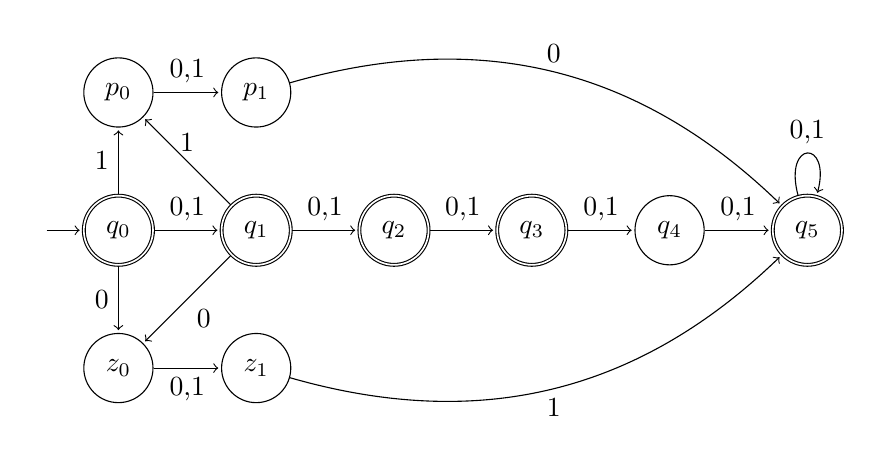
\begin{tikzpicture}[shorten >=1pt,node distance=1.75cm,on grid,auto,initial text=]
    \node[state,initial,accepting]   (q_0)                {$q_0$};
    \node[state,accepting]           (q_1) [right=of q_0] {$q_1$};
    \node[state,accepting]           (q_2) [right=of q_1] {$q_2$};
    \node[state,accepting]           (q_3) [right=of q_2] {$q_3$};
    \node[state]                     (q_4) [right=of q_3] {$q_4$};
    \node[state,accepting]           (q_5) [right=of q_4] {$q_5$};
    \node[state]                     (p_0) [above=of q_0] {$p_0$};
    \node[state]                     (p_1) [right=of p_0] {$p_1$};
    \node[state]                     (z_0) [below=of q_0] {$z_0$};
    \node[state]                     (z_1) [right=of z_0] {$z_1$};
    \path[->]
     (q_0)   edge                node {0,1} (q_1)
     (q_1)   edge                node {0,1} (q_2)
     (q_2)   edge                node {0,1} (q_3)
     (q_3)   edge                node {0,1} (q_4)
     (q_0)   edge                node {1}   (p_0)
     (q_1)   edge                node[above] {1}   (p_0)
     (q_0)   edge                node[left] {0}   (z_0)
     (q_1)   edge                node {0}   (z_0)
     (q_4)   edge                node {0,1} (q_5)
     (p_0)   edge                node {0,1} (p_1)
     (z_0)   edge                node[below] {0,1} (z_1)
     (p_1)   edge [bend left, above] node {0}   (q_5)
     (z_1)   edge [bend right, below] node {1}   (q_5)
     (q_5)   edge [loop above]   node {0,1} (q_5);
 \end{tikzpicture}

(a) For each state $q \in Q$, describe the set of strings $w \in \{0,1\}^*$ such that $q \in  \de^*(q_0, w)$.\\
Your descriptions should not mention $\delta$.

\tbf{Description.} Let $k\in\Z^+$ be arbitrary. By definition of $\de^*$, it is equivalent to describe for each $q\in Q$, what strings $w\in\{0,1\}^*$ will lead to state $q$ from the initial state $q_0$. We will prove our description in part (b).

Now, if $q=q_i$ for some $i\in[2k]\cup\{0\}$ (we instantiate such $i$), then $q$ can be reached from $q_0$ by a string $w\in\{0,1\}^*$ if and only if $w$ is a string with length $i$.

If $q=q_{2k+1}$, there are 2 cases that the string will reach $q_{2k+1}$: First, any string $w\in\{0,1\}^*$ with length at least $2k+1$ will reach $q_{2k+1}$; Second, if $w\in\{0,1\}^*$ has length at least $k+1$, and there exists 2 letters $a\in w$, $b\in w$ such that $a\ne b$ and they are $k-1$ letters apart, then $w$ will reach $q_{2k+1}$ (by ``$\in$'' we mean $a$ is one of the letters of the string $w$, etc).

Let $\om=\{w\in\{0,1\}^*\mid \T{ $w$ has length at most $k-1$}\}$.

For $p_0$, if $w=w'\cd 1$ for some $w'\in\om$, then $w$ will reach $p_0$; For $p_i$ with $i\in[k-1]$, if $w=w'\cd 1\cd w''$ for some $w'\in\om$ and $w''\in\{0,1\}^{i}$, then $w$ will reach $p_i$.

Similarly, for $z_0$, if $w=w'\cd 0$ for some $w'\in\om$, then $w$ will reach $z_0$; For $z_i$ with $i\in[k-1]$, if $w=w'\cd 0\cd w''$ for some $w'\in\om$ and $w''\in\{0,1\}^{i}$, then $w$ will reach $z_i$.

% First since all $q_i$ where $i\in[2k+1]\cup\{0\}-\{2k\}$ are final states, we can see all strings that have length not equal to $2k$ will be accepted. 

% Now we focus on strings $w\in\{0,1\}^*$ with length $2k$. Let $w\in\{0,1\}^{2k}$ be arbitrary, then we can think $w$ as a concatenation of $w=p\cd q$ where $p\in\{0,1\}^k$ and $q\in\{0,1\}^k$. We claim that string $w$ with length $2k$ is accepted

(b) Prove that $L(N_k) = X_k$ for all $k \in \ints^+$.

\tit{Proof of Question 2(b).}

\indenv{
    Let $k\in\Z^+$ be arbitrary.
    \indenv{
        Let $w\in\{0,1\}^*$ be arbitrary.
        
        Consider 3 cases of the length of $w$: $|w| < 2k, |w|=2k, |w|>2k$.

        \begin{proofcases}
            \case $|w| < 2k$.
            \indenv{
                Since $\de(q_i,0)=\{q_{i+1},z_0\}$ and $\de(q_i,1)=\{q_{i+1},p_0\}$ for $0\le i \le k-1$, and $\de(q_i,0)=\de(q_i,1)=\{q_{i+1}\}$ for $k\le i\le 2k$, from these we have $q_{i+1}\in\de(q_i,\al)$ for $0\le i\le 2k$ where $\al\in\{0,1\}$.
            }
        \end{proofcases}
    }
}




\end{document}